In this section, we present SQLiteKV and its detailed design architecture. SQLiteKV is a variant of LSM tree-based key value storage engine, like Google's LevelDB or Facebook's Cassandra. It is augmented with two layers and four modules. The front-end layer includes a SQL-to-KV compiler, from which existing applications could migrate from SQLite to key-value storage without any modifications on their original SQLite codes, as well as a slab-allocation caching for memory efficiency and de-fragmentation. At the back-end layer of SQLiteKV, a new index management scheme is proposed to work along with the underlying LSM-tree-based storage engine. It can significantly improve the performance and scalability of meta-data management as well. 

\section{Design Overview}
\begin{figure}[h]
	\centering
	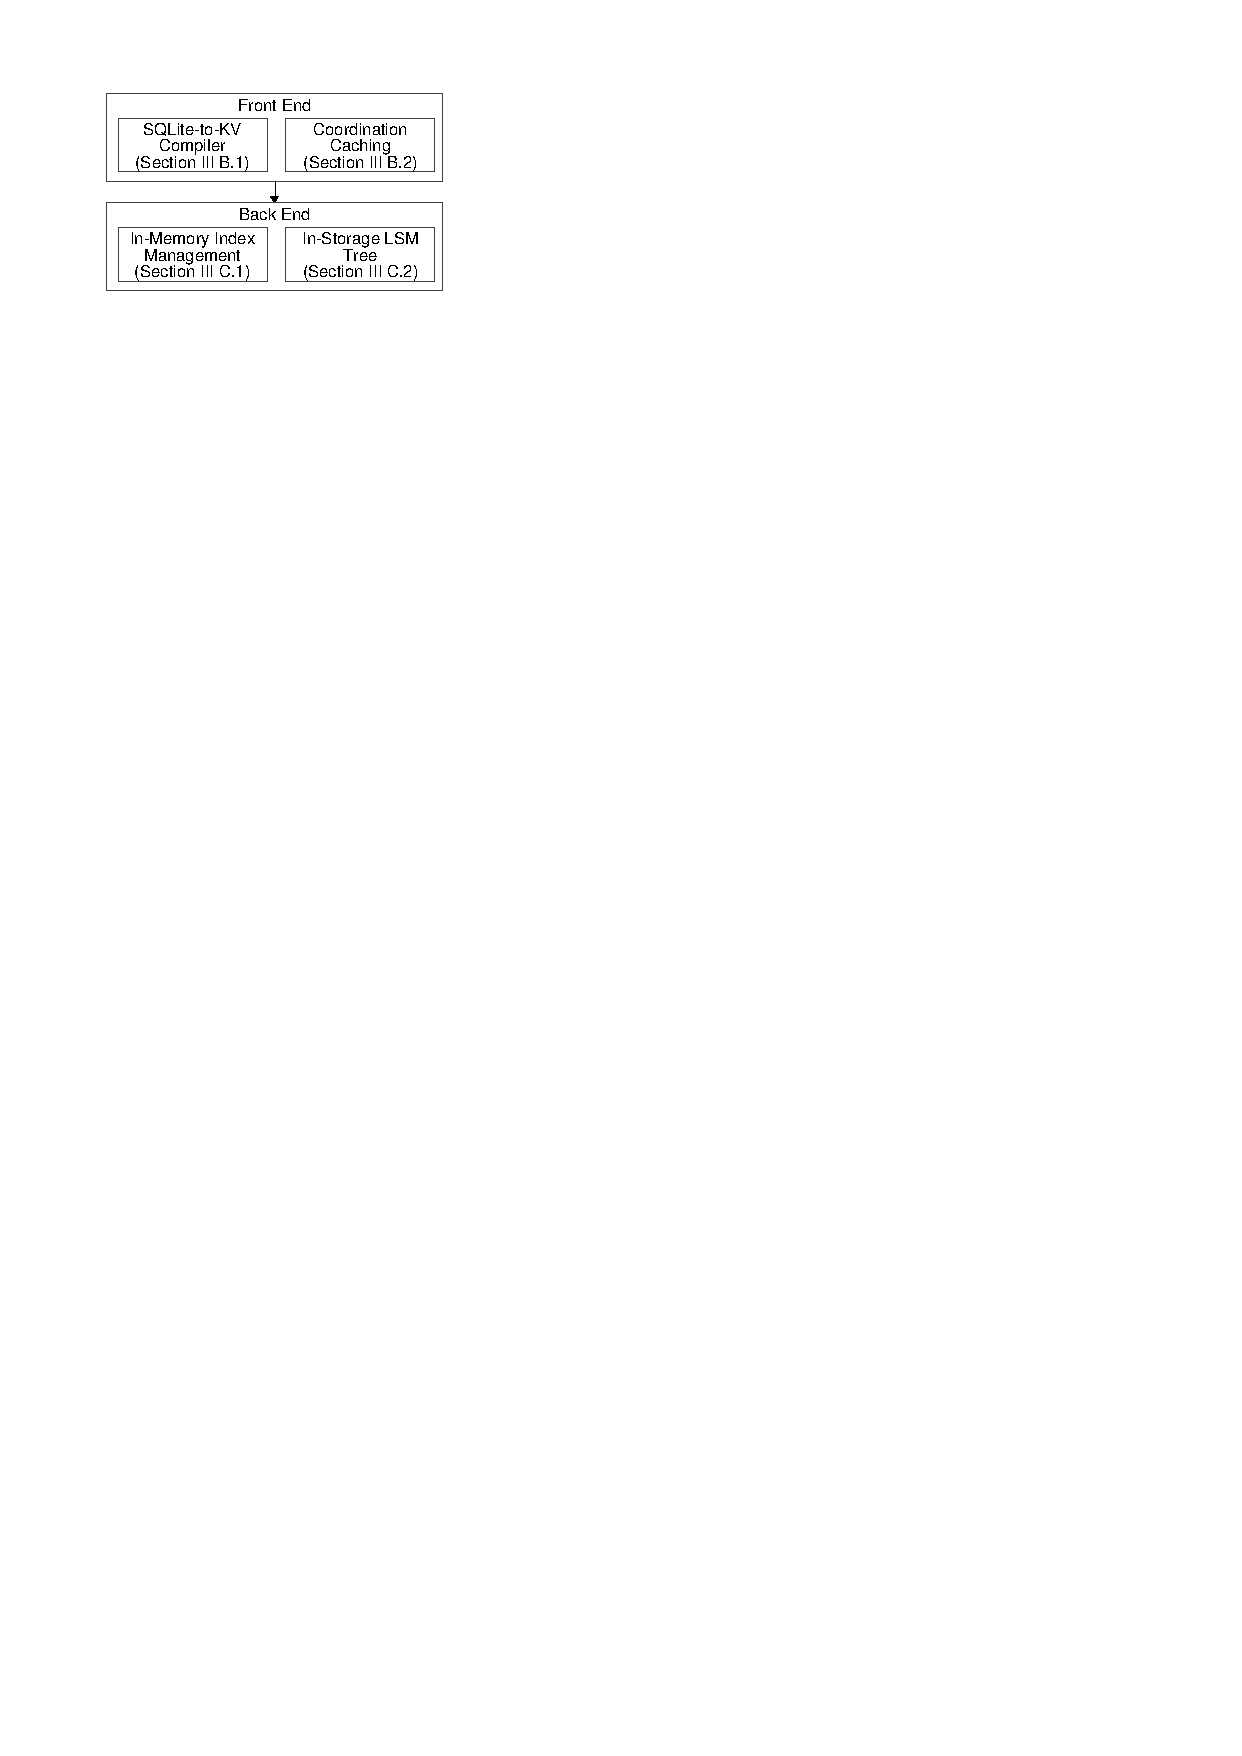
\includegraphics[width=0.4\textwidth]{pic/SQLiteKV.pdf}
	\caption{Architecture of SQLiteKV.}
	\label{fig:SQLiteKV}
	\centering
\end{figure}
As shown in Fig ~\ref{fig:SQLiteKV}, SQLiteKV is augmented with two layers, the front-end layer and the back-end layer. Front-end layer consists of two modules: a SQLite to KV compiler and a slab-allocation caching. As energy optimization is of vital importance in mobile devices and memory contributes to a large portion of total energy consumption of embedded devices \cite{shao2012utilizing},  our back-end layer  mainly focus on the memory and storage optimization. The two main modules of it are a re-designed index management and a LSM-tree based storage engine. 

The overall architecture and these functional modules are illustrated in Figure~\ref{fig:SQLiteKV}.  The two layers with four functional modules are described below in more details.
\subsection{Front-End}
	In order to provide a SQLite-Compatible interface, two major components are designed and implemented on the front-side of SQLiteKV. Fig ~\ref{fig:SQLite2KVCompiler} shows the first one-a SQLite-like interface and the second one, a slab-allocation caching mechanism, is presented in Fig ~\ref{fig:cache}.
	\subsubsection{SQLite-Like Compiler}
	\begin{figure}[h]
		\centering
		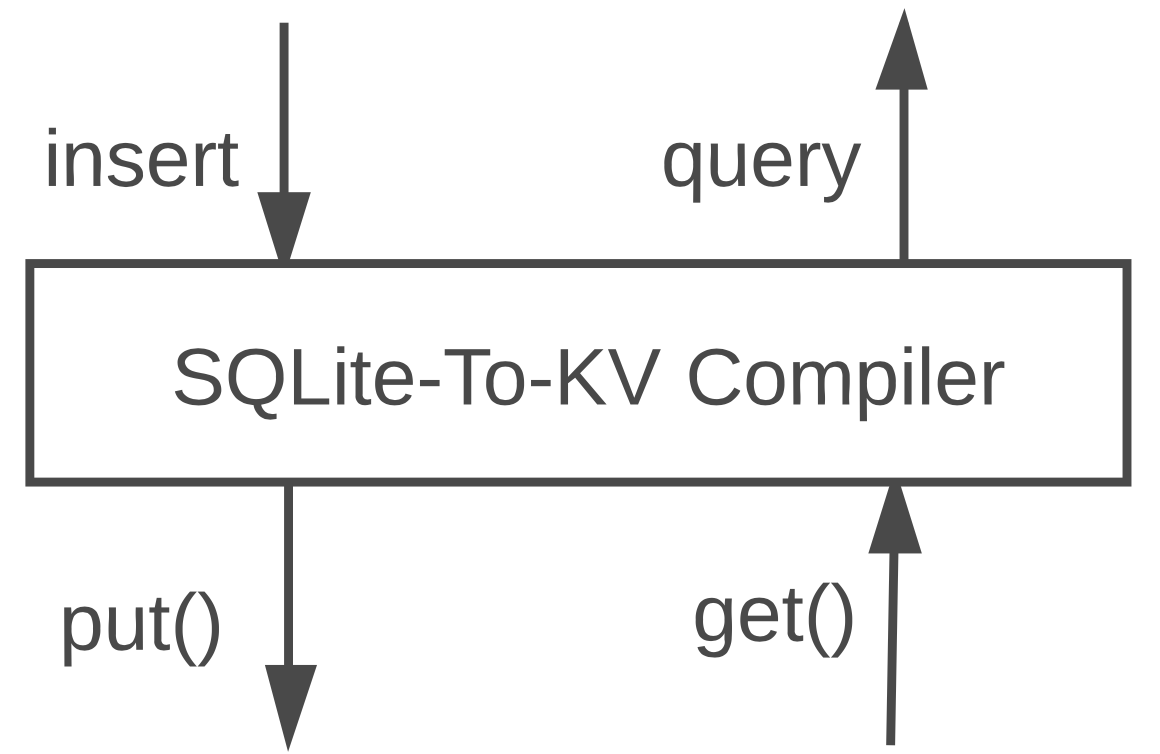
\includegraphics[width=0.35\textwidth]{pic/SQLite2KV.png}
		\caption{SQLite to KV Compiler work flow.}
		\label{fig:SQLite2KVCompiler}
		\centering
	\end{figure}
 	As for the interpretation of SQL statements, our SQLite-to-KV compiler firstly breaks down the statements into tokens. Then it would give each token meaning based on the context and assemble it into a parser tree. So far the compilation goes similarly as SQLite. The most important step is that it would generate key-value operations based on the result of parsing. Generally, there would be three kind of operations including GET(), PUT()  and DELETE(), which is also a common feature among NoSQL database. KV operations will be passed to and executed in the back-end storage engine.
	
	This SQLite-to-KV compiler makes it possibile that existing applications could run smoothly with original SQL statements and leverage the potentials of key value storage.
	
	\subsubsection{Slab-Allocation Caching}
		\begin{figure}
		\centering
		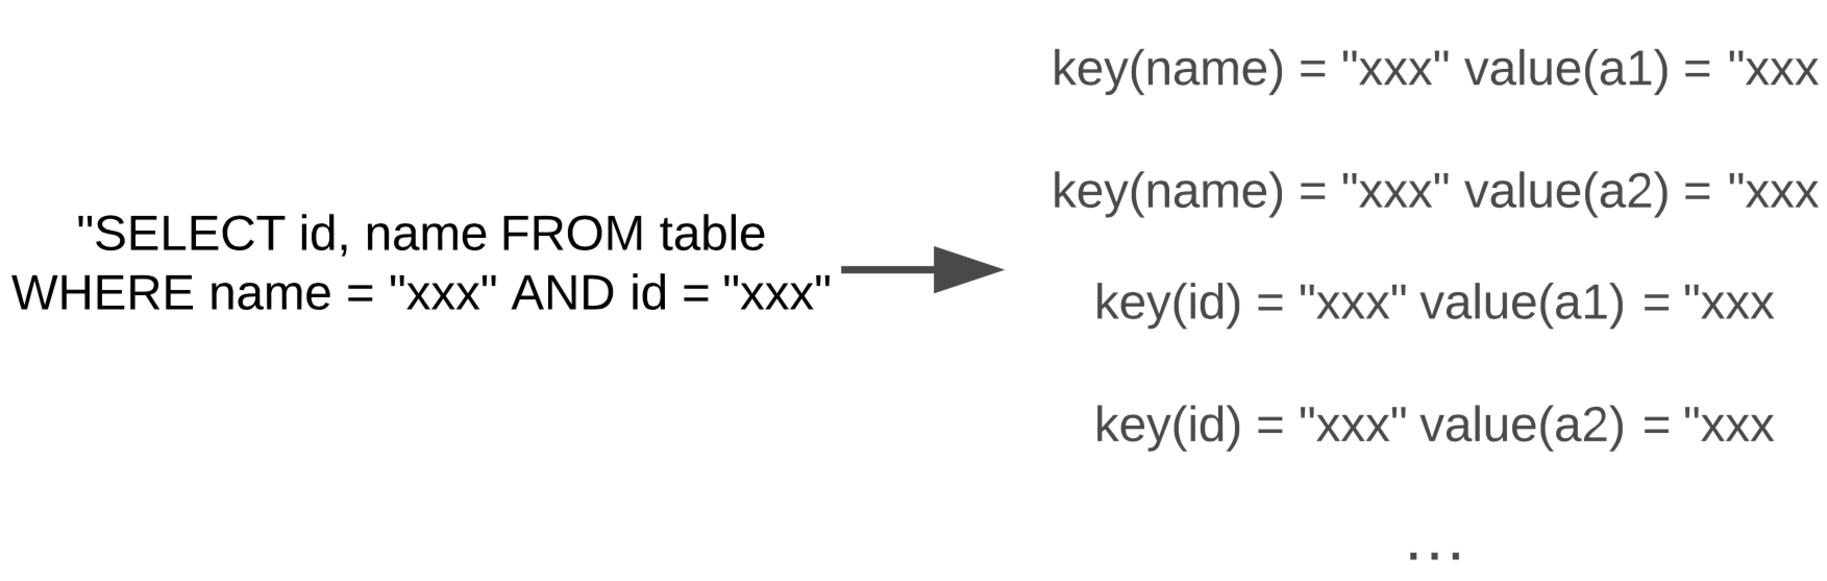
\includegraphics[width=0.6\textwidth]{pic/Cache-eg.pdf}
		\caption{One Single SQL to Multi KV items.}
		\label{fig:CacheEG}
	\end{figure}
		\begin{figure}[h]
			\centering
			\begin{subfigure}[b]{0.35\textwidth}
				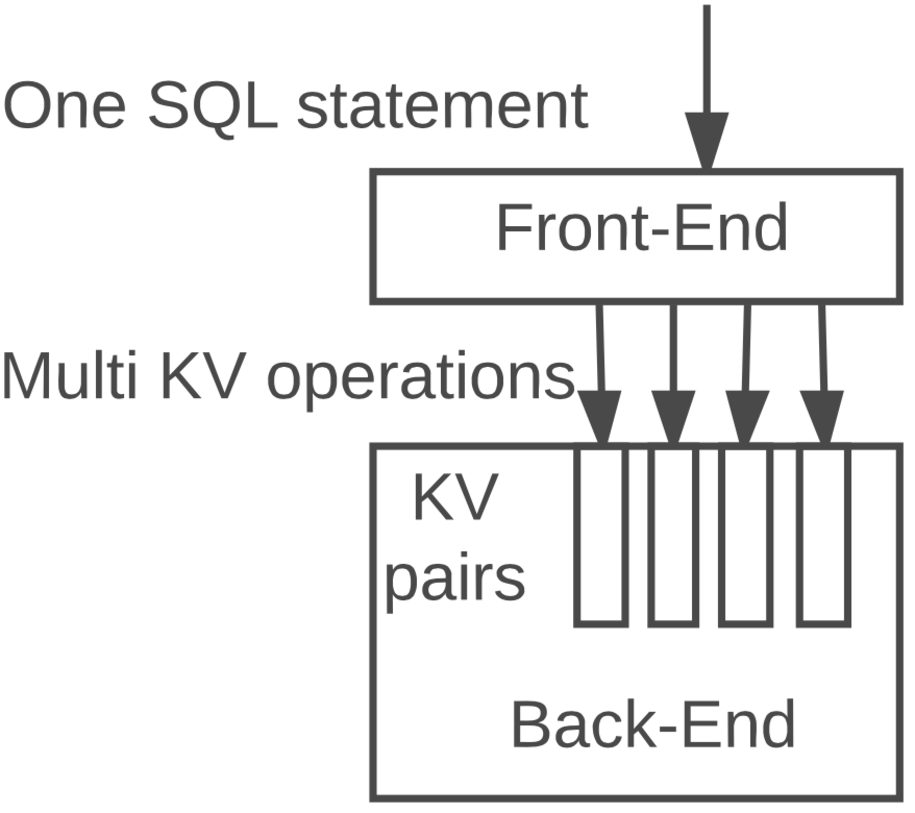
\includegraphics[width=\textwidth]{pic/KVCache.pdf}
				\caption{SQLiteKV without Cache.}
				\label{fig:KVCache}
			\end{subfigure}
		\begin{subfigure}[b]{0.35\textwidth}
			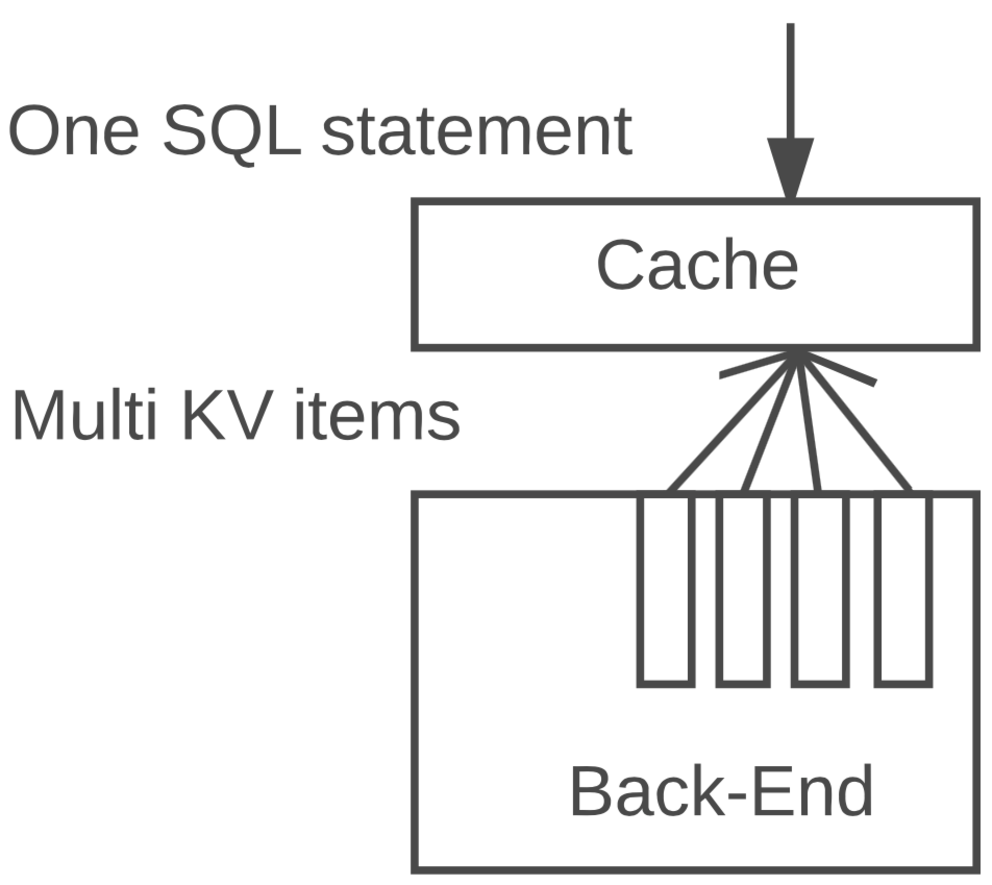
\includegraphics[width=\textwidth]{pic/SQLiteKVCache.pdf}
			\caption{SQLiteKV with Cache.}
			\label{fig:SQLiteKVcache}
		\end{subfigure}
	\caption{SQLite Slab-Allocation Caching}
	\label{fig:cache}
	\end{figure}
	 SQLite uses a caching mechanism inside its back end engine to cache frequently-visited pages within the flash memory to avoid frequent visits to the disk. SnappyDB also implements a caching system for latest recently used KV items. However, one SQL statement usually corresponds to multi-KV items during the SQL compilation process of SQLiteKV. Neither of these above-mentioned caching could alleviate such data discrepancy between SQL statements and KV items. Therefore, we design a new caching mechanism as part of the front-end of SQLiteKV. It caches query results for SQL statements as a batch of KV items. Such mapping between SQL statement and KV items can significantly reduce the data discrepancy and improve the query performance.
	 \begin{figure}
	 	\centering
	 	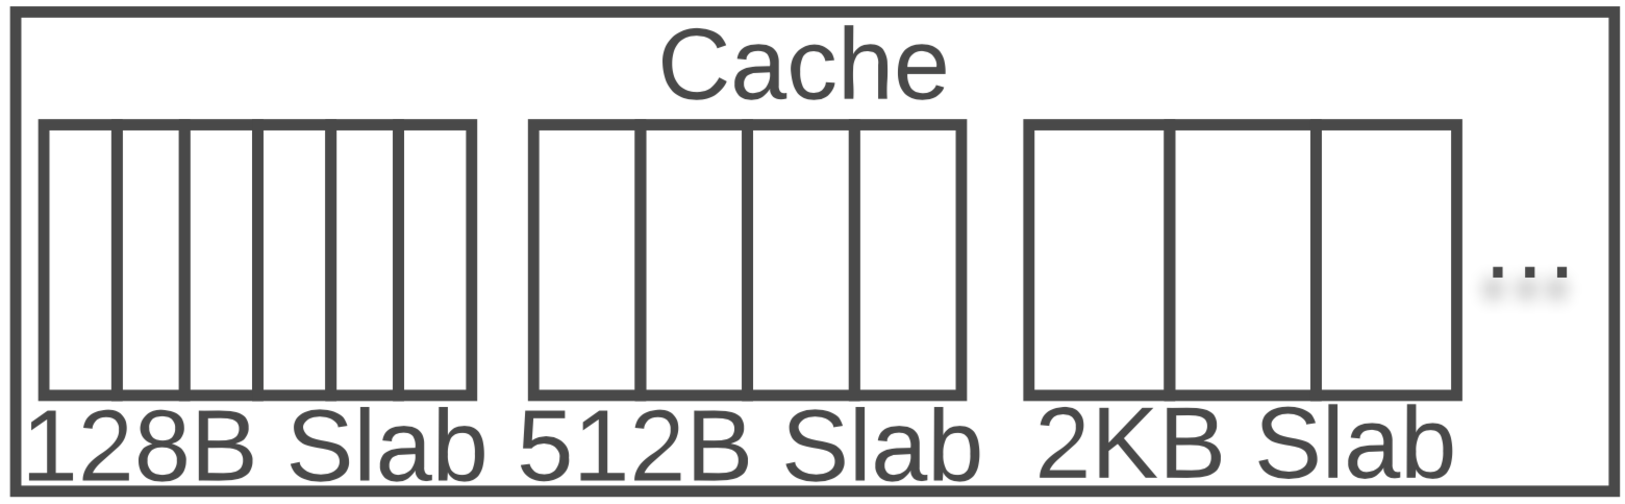
\includegraphics[width=0.3\textwidth]{pic/SQLiteKVCache2.pdf}
	 	\caption{SQLiteKV Cache Structure.}
	 	\label{fig:SQLiteCache2}
	 	\centering
	 \end{figure}
	 Moreover, a slab-allocation structure, as shown in Fig. \ref{fig:SQLiteCache2} is deployed to solve the memory fragmentation issue caused by small KV items. The slab-based caching mechanism would separate memory space into different slabs with various entry sizes, like 128 bytes, 512 bytes or 4096 bytes. A specific KV item would be cached into a slab whose size fits the itself the most. Such design can effectively address the issue of memory fragmentation, especially on embedded memory constraints devices.

\subsection{Back-End}
	\subsubsection{Index Management On LSM Tree}

 	LSM-based storage engines would commonly do a scan over the entire disk and collect all indexes back to the memory \cite{190528}. Usually index is put at the end of each data block. Hence when a query operation is to be executed, the in-memory meta-data would be binary-searched with the target key to locate the data block on disk. That data block would be visited upon then which means at most one disk seek is required for a single query on LSM-tree-based KV engine. 
 			\begin{figure}
 		\centering
 		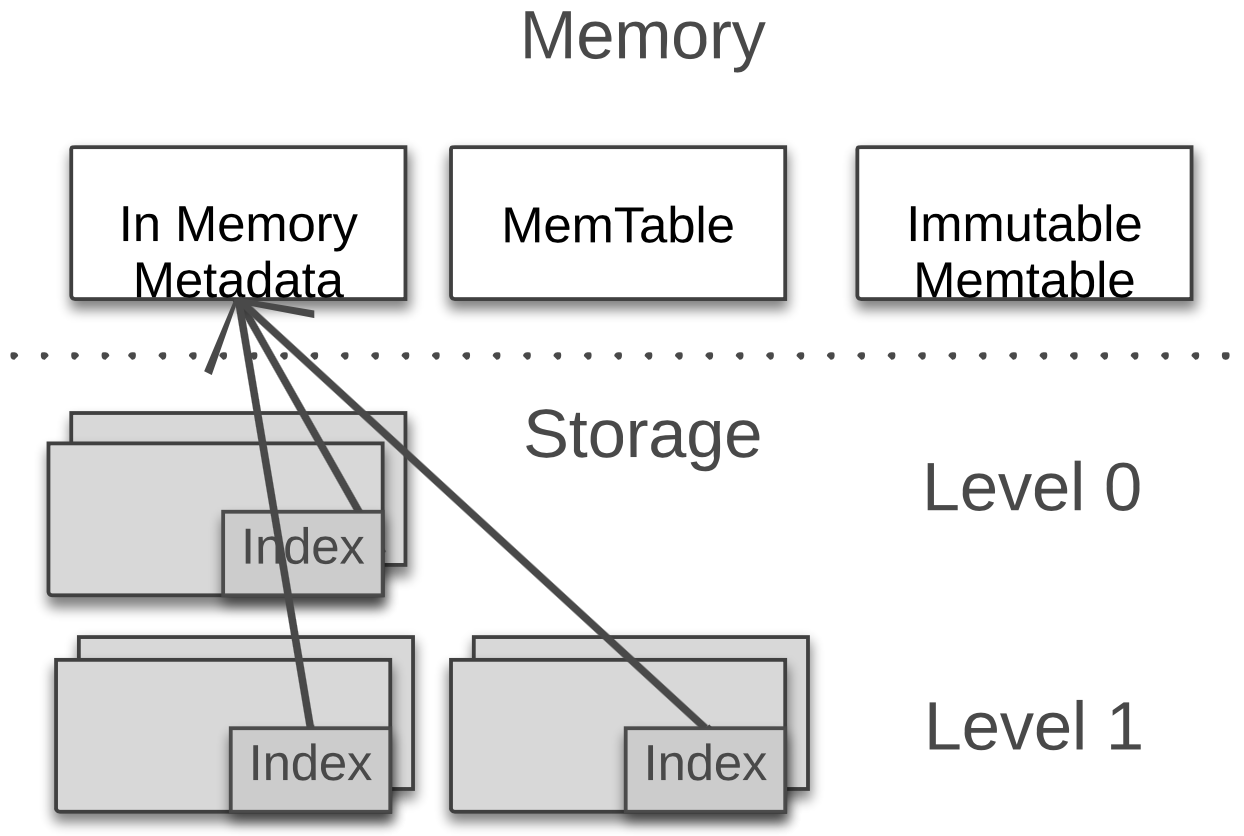
\includegraphics[width=0.35\textwidth]{pic/Back-Index.png}
 		\caption{Back-End In-Memory Index Management.}
 		\label{fig:back-index}
 		\centering
 	\end{figure}
 	However, this approach doesn't seem to be practical nor efficient since most mobile devices are memory constraints and not all the indexes could be accommodated in the memory. In accordance to this issue, we re-design the indexing management scheme, which exclusively stores indexes of data blocks in higher levels, like level 0 and 1, of the entire LSM tree. The reason is that with the level goes further down, data at lower level are less likely to be visited. In other words, the data on top levels are more likely to be newly-added or frequently-visited. Our approach reduce the huge overhead on SnappyDB's original in-memory meta-data management. At the same time, the worst disk seek time remains at same order of complexity. To sum up, our meta-data management strategy does leverage the LSM-tree structure and avoid possible memory constraints issue on the back-end side.
	
	\subsubsection{Storage Management}
		\begin{figure}[h]
		\centering
		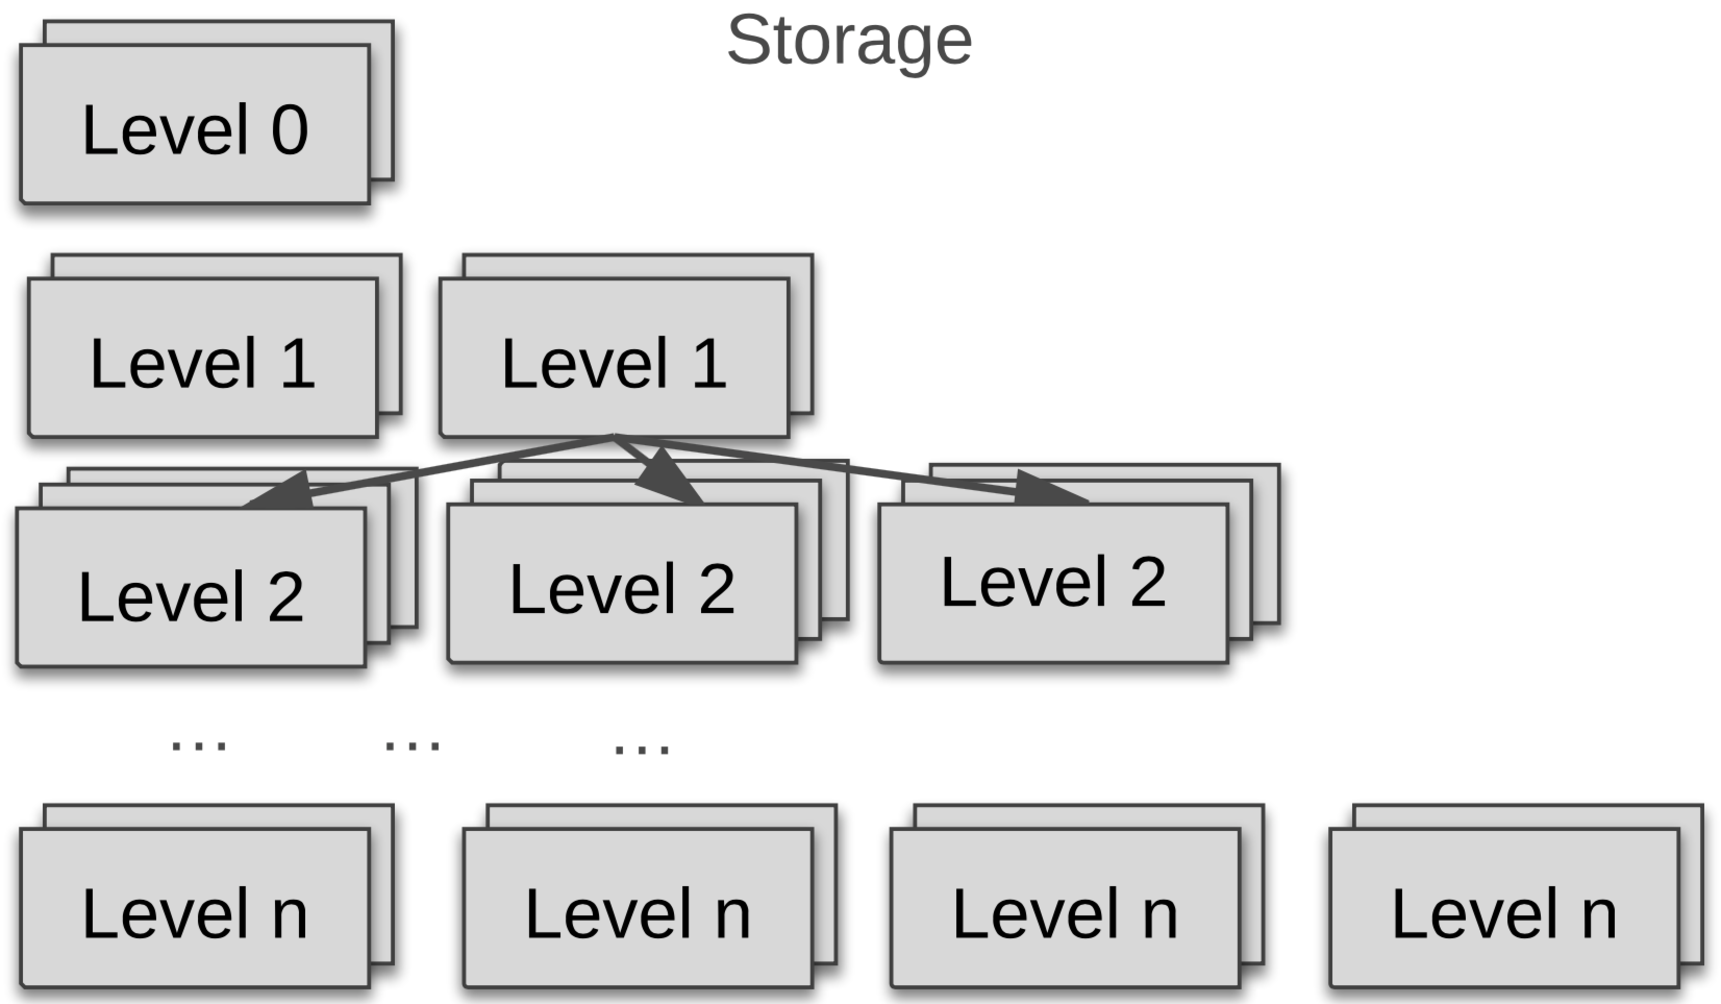
\includegraphics[width=0.32\textwidth]{pic/Back-Disk.pdf}
		\caption{Back-End Storage Management.}
		\label{fig:BackDisk}
		\centering
	\end{figure}

	The disk storage management of SQLiteKV relies mainly on its LSM-tree-based structure. As we mentioned before, once the MemTable, as shown in Fig ~\ref{fig:back-index}, is converted to be an immutable table and dumped into disk. This SSTable would be placed at the first level, level 0. As long as one specific level of this LSM tree is full, those SSTables with overlapping indexes would be compacted together and dumped to the next level. During this compaction process, newly-generated SSTables on lower levels tend to have larger  sizes and ranges of index consequently. 
